\documentclass[a4]{article}
\usepackage[utf8]{inputenc}
\usepackage[french]{babel}
\usepackage{listings}
\usepackage{color}
\usepackage{graphicx}
\usepackage[T1]{fontenc}
\usepackage{pdfpages}
\usepackage{geometry}
\geometry{hmargin=2.5cm,vmargin=2.5cm}

\definecolor{mygreen}{rgb}{0,0.6,0}
\definecolor{mygray}{rgb}{0.5,0.5,0.5}
\definecolor{mymauve}{rgb}{0.58,0,0.82}

\lstset{
  backgroundcolor=\color{white},   % choose the background color; you must add \usepackage{color} or \usepackage{xcolor}
  basicstyle=\footnotesize,        % the size of the fonts that are used for the code
  breakatwhitespace=false,         % sets if automatic breaks should only happen at whitespace
  breaklines=true,                 % sets automatic line breaking
  captionpos=b,                    % sets the caption-position to bottom
  commentstyle=\color{mygreen},    % comment style
  deletekeywords={...},            % if you want to delete keywords from the given language
  escapeinside={\%*}{*)},          % if you want to add LaTeX within your code
  extendedchars=true,              % lets you use non-ASCII characters; for 8-bits encodings only, does not work with UTF-8
  frame=L,	                       % adds a frame around the code
  keepspaces=true,                 % keeps spaces in text, useful for keeping indentation of code (possibly needs columns=flexible)
  keywordstyle=\color{blue},       % keyword style
  language=C,                 	   % the language of the code
  otherkeywords={*,...},           % if you want to add more keywords to the set
  numbers=none,                    % where to put the line-numbers; possible values are (none, left, right)
  numbersep=5pt,                   % how far the line-numbers are from the code
  numberstyle=\tiny\color{mygray}, % the style that is used for the line-numbers
  rulecolor=\color{black},         % if not set, the frame-color may be changed on line-breaks within not-black text (e.g. comments (green here))
  showspaces=false,                % show spaces everywhere adding particular underscores; it overrides 'showstringspaces'
  showstringspaces=false,          % underline spaces within strings only
  showtabs=false,                  % show tabs within strings adding particular underscores
  stepnumber=2,                    % the step between two line-numbers. If it's 1, each line will be numbered
  stringstyle=\color{mymauve},     % string literal style
  tabsize=2,	                   % sets default tabsize to 2 spaces
  title=\lstname                   % show the filename of files included with \lstinputlisting; also try caption= instead of title
}
%gestion des caractères latins
\lstset{literate=
  {á}{{\'a}}1 {é}{{\'e}}1 {í}{{\'i}}1 {ó}{{\'o}}1 {ú}{{\'u}}1
  {Á}{{\'A}}1 {É}{{\'E}}1 {Í}{{\'I}}1 {Ó}{{\'O}}1 {Ú}{{\'U}}1
  {à}{{\`a}}1 {è}{{\`e}}1 {ì}{{\`i}}1 {ò}{{\`o}}1 {ù}{{\`u}}1
  {À}{{\`A}}1 {È}{{\'E}}1 {Ì}{{\`I}}1 {Ò}{{\`O}}1 {Ù}{{\`U}}1
  {ä}{{\"a}}1 {ë}{{\"e}}1 {ï}{{\"i}}1 {ö}{{\"o}}1 {ü}{{\"u}}1
  {Ä}{{\"A}}1 {Ë}{{\"E}}1 {Ï}{{\"I}}1 {Ö}{{\"O}}1 {Ü}{{\"U}}1
  {â}{{\^a}}1 {ê}{{\^e}}1 {î}{{\^i}}1 {ô}{{\^o}}1 {û}{{\^u}}1
  {Â}{{\^A}}1 {Ê}{{\^E}}1 {Î}{{\^I}}1 {Ô}{{\^O}}1 {Û}{{\^U}}1
  {œ}{{\oe}}1 {Œ}{{\OE}}1 {æ}{{\ae}}1 {Æ}{{\AE}}1 {ß}{{\ss}}1
  {ű}{{\H{u}}}1 {Ű}{{\H{U}}}1 {ő}{{\H{o}}}1 {Ő}{{\H{O}}}1
  {ç}{{\c c}}1 {Ç}{{\c C}}1 {ø}{{\o}}1 {å}{{\r a}}1 {Å}{{\r A}}1
  {€}{{\EUR}}1 {£}{{\pounds}}1
}
%definition d'un syle pour les documents text
\lstdefinestyle{txt}{
	frame=none,
	numbers=none,
	stringstyle=\color{black},
}

\begin{document}
	\title{\Huge{\textbf{Rapport Final}}}
	\author{Alabi Steve - Benyamna Younes - Capdenat Nicolas- \\
		Chouipe Thibaut - El Harti Zakaria - Lienhardt Florian \\ \\ \\
		Chef de projet : Benyamna Younes \\ \\ \\ 
		Sous la direction de Mme Kloul \\ \\ \\ \\
		Outil automatique de décryptage \\ \\ \\}
	\date{29 mai 2017}
		

	\begin{titlepage}
		\maketitle
		\vspace{20em}
		%\begin{center}
\includegraphics{logo_uvsq.jpg}\end{center}
	\end{titlepage}
	\section{Introduction}
Après avoir réalisé le cahier des charges, qui exprime les besoins/attentes du client ainsi que
les contraintes a respecter, et après avoir decrit comment les exigences fonctionnelles vont être implémentées(cahier des specifications)
, nous nous sommes donc lancés dans la réalisation du produit. \\ \\
Dcrypt est maintenant disponible et utilisable par le client. Un manuel d'utilisation
détaillé lui sera egalement fournit pour expliquer le fonctionnement de l'application.\\

Dans ce rapport, il s'agira de s'interesser tout d'abord à la logique/architecture de l'application et au choix du langage.
Enfin, nous pouvons nous pencher sur la partie technique du produit.
Pour cela, nous montrerons le fonctionnement de l'application à l'aide de tests, puis nous parlerons de l'organisation interne
 et pour finir nous verrons la comparaison du nombre de lignes de code réelles avec les estimations faites dans le cahier des charges.


	\section{Objectif de l'application}
	
	
	Le but du projet est donc de developper un logiciel pour automatiser le decryptage d'un texte.
	Le produit est réalisé afin de satisfaire le client, et pour se faire il doit répondre à toutes ses attentes.\\
	Ainsi, le client peut crypter ou decrypter un texte ou fichier et ce par methode de Substitution ou Vigenère.
	Mais aussi, il lui est possible d'effectuer independamment une analyse frequentielle sur un texte donné.
	
	

	\section{Architecture de l'application}
			\underline{Interface graphique :}     \hspace{5cm}  \underline{Cryptage Substitution :}\\
			- bouton cryptage            \hspace{5.5cm}       -créer une clé aleatoirement\\
			- bouton decryptage         \hspace{5cm}        -crypter le message\\
			- bouton substitution\\
			- bouton Vigenère           \hspace{5.2cm}       \underline{Cryptage Vigenère :}\\
			- affichage de texte(complet et partiel)  \hspace{2.2cm} -crypter le message\\
			- affichage pour la clé de substitution\\
			- bouton Francais(decryptage)   \hspace{3.5cm}     \underline{Decryptage Substitution :}\\
			- bouton Anglais(decryptage)    \hspace{3.5cm}     -decrypter le message\\
			- affichage pour l'analyse fréquentielle\\
			- charger un fichier texte       \hspace{4.2cm}  \underline{Analyse fréquentielle :}\\
			- sauvegarder un fichier texte     \hspace{3.8cm}  -analyse frequentielle sur texte donné\\
			- créer un nouveau fichier texte(resultats)\\
			- Demander clef de Vigenère\\
			
			\underline{Decryptage Vigenère :}\\
			-decrypter le message\\
			
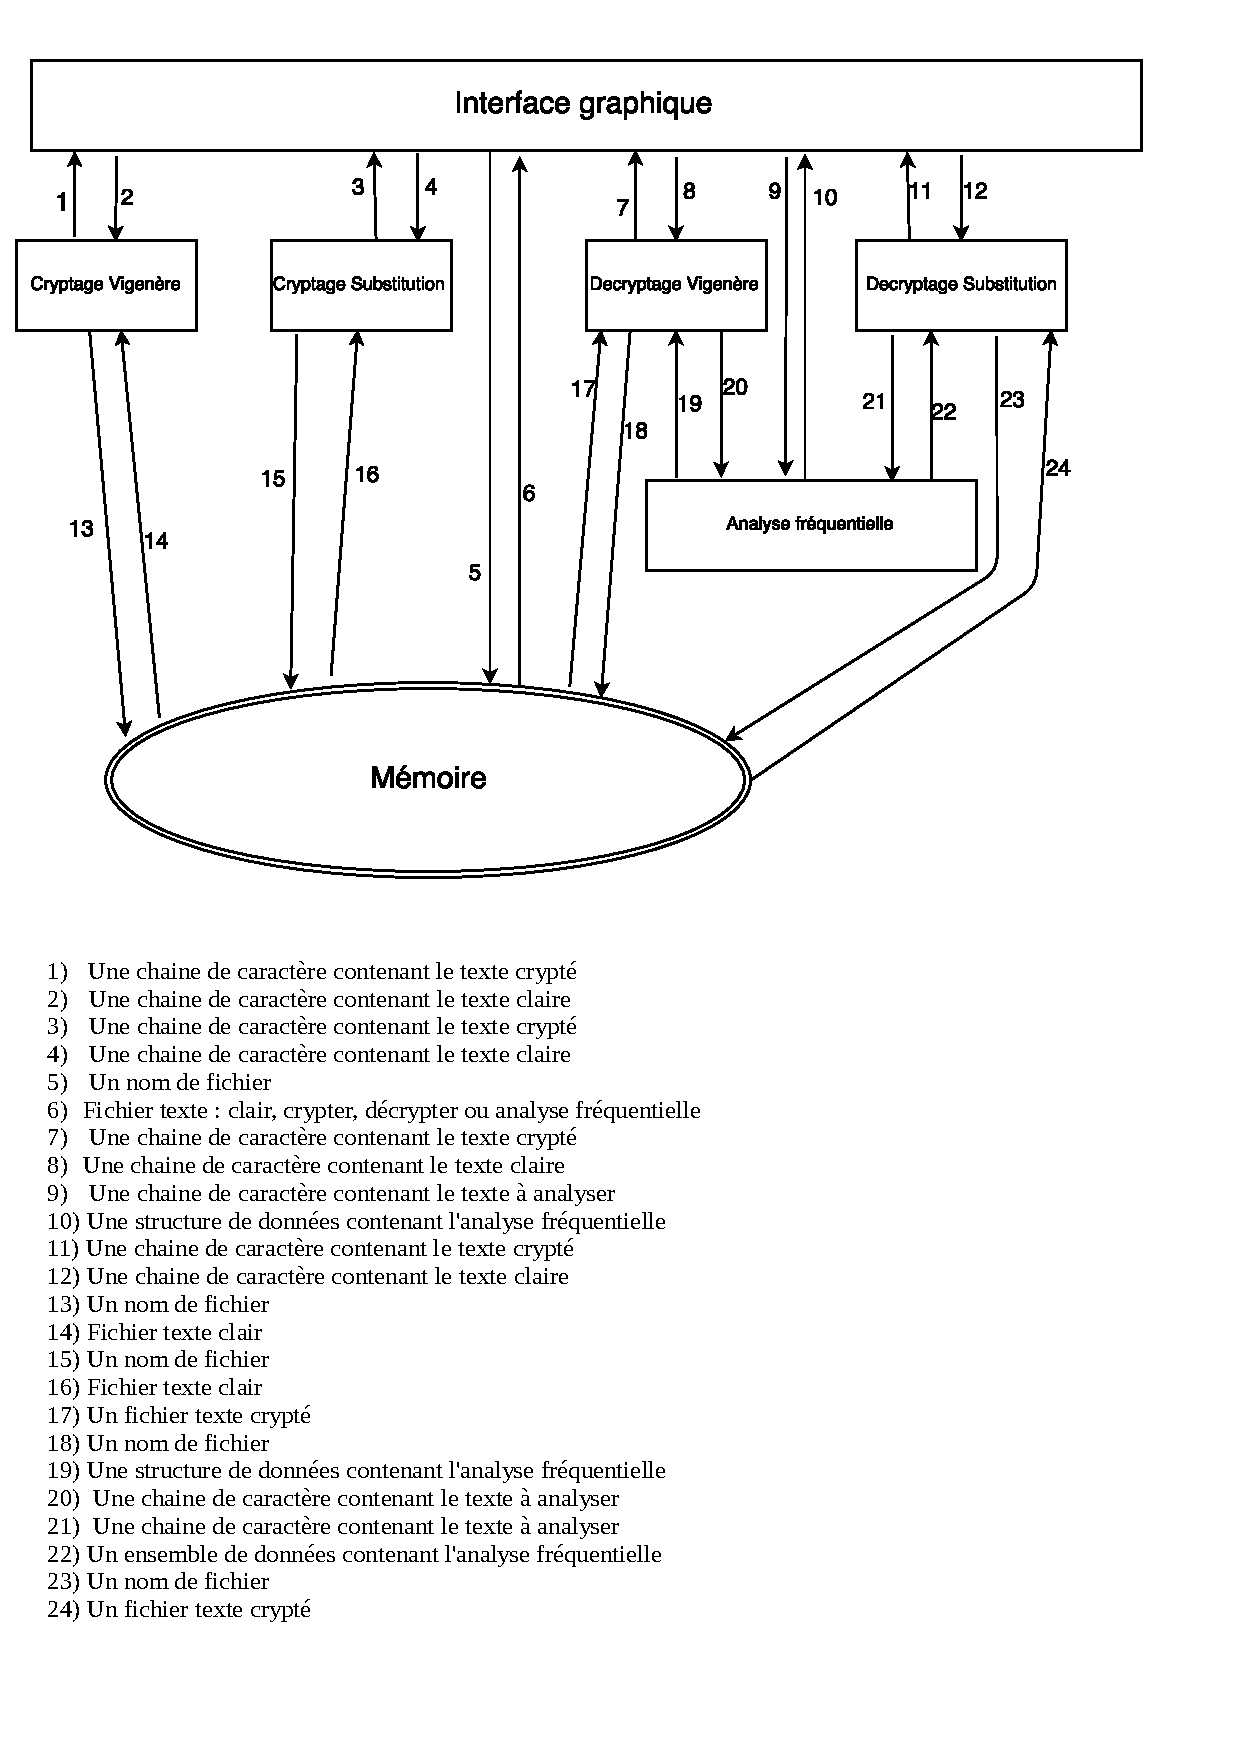
\includepdf[scale=0.9]{organ.pdf}
			
			EXPLICATION DE L'ORGANIGRAMME ICI \\ \\ \\ \\ \\ \\ \\ \\ \\
	\section{Language choisi et explications}
	
	Le developpement de l'application s'est fait en langage C et les raisons étant les suivantes: \\
	
Nous avions besoin d'une application fonctionnelle et donc d'un langage procédurale. Le meilleur langage sur le marché
etant le C, le choix s'est logiquement porté sur ce dernier.\\ \\

Aussi, un argument de choix est celui de la portabilité. En effet, nous avions besoin d'une portabilité sur plusieurs
environnements et donc d'un besoin de standard ou norme. D'ou le langage C, car en effet il est possible d'utiliser
 le même programme sur tout autre système
 (autre hardware, autre système d'exploitation), simplement en le recompilant. \\ \\ \\



La bibliothèque graphique que nous avons décidée d'utiliser avec ce langage est GTK+ 
		parce qu'elle permet d'implémenter des boutons, des zones de texte, des menus ou encore du traitement de fichier.
		Elle nous semblait donc la plus adaptée au developement de notre application.
	\section{Partie technique}
	
	Tout d'abord, l'application fonctionne (compilation et execution) et
	l'ensemble des fonctionnnalités demandées par le client ont été réalisées.\\ \\
	
	Nous souhaitions avoir une application complète qui puisse tourner sur des ordinateurs 
de tout systeme d'exploitation et ce, sans pour autant qu’il ne
consomme trop de mémoire ou de temps processeur. \\ \\
	
	L'equipe de developpement a evidemment rencontré bon nombre de problèmes ou bugs. Voici une liste non exhaustive: \\
	-probleme du switch, remplacé par if (younes nicolas)\\
	-probleme de segfault du a la gestion de la memoire: remplace "gchar* exemple" par "gchar exemple[10]" (zak) \\
	-\\
	-\\ \\
		
		
		-Des approximations et des erreurs de jugement sur le cahier des specifications ont conduit a certains changements ou problemes:
		-\\
		-\\
		-\\
		-\\ \\
		
		
		
		

		La decoupe technique des modules s'est faite en fonction des fonctionnalités.
		 Chacune de ces dernieres correspondant a un module.
		
		\subsection{Tests (unitaires)}
		L’exactitude des resultats de l'analyse etant tres importante pour les clients, nous avons predefinis des tests
unitaires pour chaque module(ou plutot les fonctions le composant). Ainsi, a chaque etape de la conception du logiciel
nous avons pu verifier que le calcul n’etait pas altere. \\ \\
Les resultats des tests unitaires sont les suivants:\\ \\ 
METTRE SCREEN TESTS "RUN" ICI

		
	\section{Organisation interne et affectation des taches}
	L'organisation de l'équipe est une chose importante pour le bon fonctionnement du
projet et le deroulement du codage, et est faite selon nos capacités et nos disponibilités.  \\ \\
		-tableau des taches: qui a fais quoi?? \\
		 \includepdf[scale=0.9]{tab_taches.pdf}
		 
		 EXPLICATIONS SUR TABLEAU DES TACHES  \\	\\
		
		L'organisation etant bonne et la cohesion du groupe certaine, la repartition et la mise en place d'un planning 
		s'est faite naturellement et a été respectée.  \\
		La communication étant la clé d'un projet en groupe, nous avons préféré
		 nous reunir très regulierement et travailler tous ensemble et ce quel que soit l'etape du projet.
		\subsection{Planning de developpement}
		La phase de developpement constitue l’etape critique du projet, avec d’une part la decision de coder l’interface graphique
et d’autre part l’integration de tous les modules séparement. Lors de cette phase, les modules ont connu leurs dernieres evolutions ou plutot ajustements. \\
Avant de tester l’ensemble de l’application, nous avons dans un premier temps codé et
testé chaque fonction ou plutot module pour savoir si elles fonctionnaient séparément. \\
Nous les avons ensuite
réunies en les assemblant étapes par étapes pour construire l’application finale.  \\
--> en priorité : l'interface graphique consistait la base de l'application et devait donc être commencée et avancée tres rapidement \\
 \\ 
En evaluant les connaissances de chacun et en faisant un point regulierement sur nos taches respectives, cela a permis 
d'avancer efficacement dans la réalisation le projet.
	\section{comparaison lignes de code}
	\includepdf[scale=0.9]{tab_comp_lignes.pdf}		
		Certains modules ont depassés le nombre de lignes estimées selon les raisons suivantes: \\
		
		-decryptage Vigenere : nombre de ligne trop juste au vu de certaines fonctions qui permettent de vérifier
		 nos résultats, par exemple la taille du mot clé. \\
		-cryptage substitution : il faut une fonction(tirage) qui va permettre qu'une lettre est toujours chiffrée
		 par une seule et meme lettre. \\
		-analyse frequentielle: fonction AnalyseFreq en plus qui est une tres legere variante de l'analyse des occurences de 
		chaque lettre faite deja dans AnalyseFrequentielle. Aussi, dans cette derniere, l'analyse des trigrammes fonctionne exactement
		comme celle des digrammes et donc on a repeté ces "autres" 40 lignes \\
		-interface graphique??
		
	
	\section{Conclusion}
	-des choix a changer \\
	->au niveau des specifications et des fonctions \\ \\
	
	-critique du projet \\
	->Manque de reflexion ou d'approfondissement de certaines notions a des moments
	->?????? \\ \\ \\
	
	
		
	-si a refaire, pareil?? \\
	->Le groupe serait le meme et la base du projet aussi. \\ \\ \\
	
	
	Finalement, nous avons une version "1.0" de l’application. La majorité des fonctionnalités
de base ont été implémentées et fonctionnent correctement mais il existe quelques
améliorations qui pourraient aboutir véritablement à une version "2.0" vraiment intéressante. \\
Quelques améliorations pourraient être ajoutées :
-Vigenere : ajout d'informations supplémentaire qui permettent d'aider/ameliorer le decryptage 
(exemple : on connait déja la taille de la clé).
-permettre a l'utilisateur de rentrer un type de texte (poeme, roman..) pour aider au decryptage \\
-plus de langues disponibles \\
-plus de cryptages/decryptages differents \\
-\\
-\\ \\ \\

	
	
Ce projet d'une durée d'un semestre(et plus precisement de X semaines) est une vrai expérience.
Cela a été enrichissant d'un point de vue personnel ou collectif:
il nous a apporté beaucoup, tant au
niveau technique qu’en terme de gestion de projet.  \\  \\
Nous connaissons maintenant l'importance du decoupage d'un projet en plusieurs etapes: cahier des charges, specifications,codage..
C'est un projet en "conditions d'entreprise" qui nous servira dans le futur.
C’est la première fois que nous travaillons en groupe a aussi nombreux sur un projet avec des caracteristiques bien définies. \\ \\
Nous sommes globalement satisfaits de ce que nous avons réalisé.
 Au niveau de la gestion du projet en équipe, nous avons réussi à bien nous répartir les
tâches afin de réaliser nos objectifs dans les temps et l'ambiance générale du groupe était très
bonne. \\ \\ \\





	
	
	
\end{document}
